% -------------------------------------------------------------------
% - NAME:        poster.tex
% - AUTHOR:      Moritz Oberracuh
% - DATE:        2019/02/26
% -------------------------------------------------------------------
% - DESCRIPTION: Preliminary results of my master thesis (importance of explicit glacier dynamics)
% presented at the AGM2019 Innsbruck on the 28 Feb. 2019
% -------------------------------------------------------------------
\pdfminorversion=4
\documentclass[final]{beamer} 

\usepackage{natbib} % citation
\usepackage{pdfpages} % include pdf documents
\usepackage{amsmath} % math package
\usepackage[english]{babel} % language package

% Specify page layout
\usepackage[orientation=portrait,size=a0,scale=1.30]{beamerposter}
\usetheme[ncols=2]{uibkposter}

%% Choose header image
\headerimage{1}

%% Set title meta data
\title{Testing the importance of explicit glacier dynamics for future glacier evolution in the Alps}
\author{Moritz Oberrauch (\textit{moritz.oberrauch@uibk.ac.at}), Fabien Maussion} 

%% Enable numbered captions (figures, tables)
\setbeamertemplate{caption}[numbered]

%% Begin document
\begin{document}
\begin{frame}[fragile]
\begin{columns}[t]

%% ----------------------------
%% begin left column for both
%% ----------------------------
\begin{leftcolumn}
   %% please leave one blank line here

   %% Introduction
   \begin{boxblock}{Volume-area scaling vs. shallow ice approximation}
      Even though the \textbf{Open Global Glacier Model (OGGM)} is a rather simple model (concerning the implemented physics), the \textbf{volume-area scaling (VAS) glacier model} originally used by \citet{Marzeion2012} is even more basic. While the OGGM implements the shallow ice approximation to drive the model glacier, the VAS model relies solely on volume/area and volume/length scaling principles.
      
      \textbf{What am I doing?!} Currently I'm implementing the original volume/area scaling model used by Ben (at least I'm trying to).
      
      \textbf{Why am I doing it?!} More complex models generelly come with higher computational costs. While this may be necessary for certain detailed analyses, not all scientific questions call for such a high degree of accuracy. In addition, alpine glaciers will most likely not advance much in the coming decades. Hence, do ice dynamics play a secondary role compared to ice melt?!

      \textbf{What do I want to achieve?!} I'd like to know, what (and how much) additional information is gained by operating a physical ice dynamics model. Or in other words, how far can I dumb the dynamic model down while still producing reasonable results on a regional  scale. This calls for the following steps:
      \begin{enumerate}
         \item Implementing glacier model(s) with different levels of complexity in the OGGM framework.
         \item Investigating strengths and weaknesses of the VAS model approach (sensitivity analysis).
         \item Completing regional runs for the alpine region (past and future).
      \end{enumerate}
   \end{boxblock} % END - Introduction

   % Scaling
   \begin{boxblock}{The scaling model}
      The model operates on an annual time step, where $t$ indecates the current year. The volume change $dV(t)$, and subsequentually next years volume \mbox{$V(t+1)$}, are computed given the specific mass balance $B(t)$ and the surface area $A(t)$. The new volume is used to estimate a equilibrium surface area $A_\text{eq}$, which then gives the actual area change $dA(t)$ by accounting for the glaciers response time $\tau_A$:
      \begin{align}
         dA(t) = \frac{1}{\tau_A(t)} \left(\underbrace{\left(\frac{V(t+1)}{c_A}\right)^{1/\gamma}}_{A_\text{eq}} - A(t)\right),
      \end{align}
      thereby $c_A$ and $\gamma$ are the volume/area scaling parameters. The length change $dL$ is computed analogously, using the corresponding parameters $c_L$ and $q$ and response time $\tau_L$.
      \begin{figure}
         \centering
         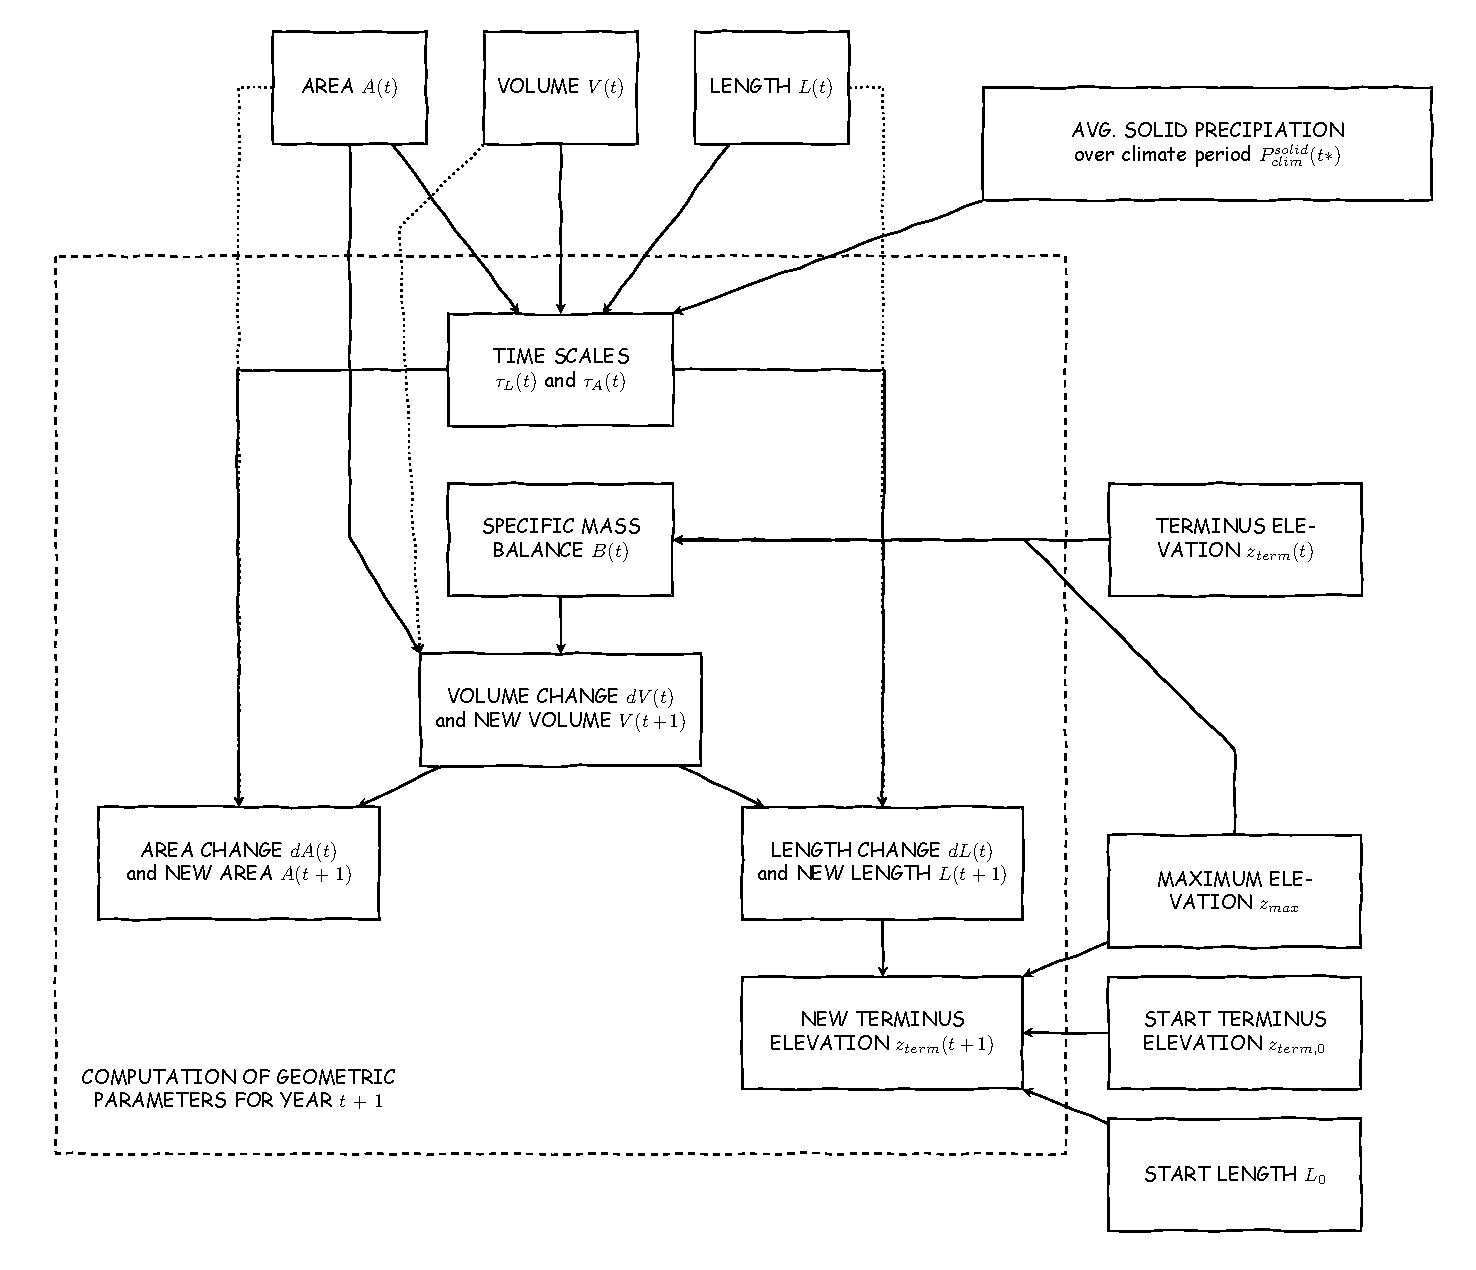
\includegraphics[width=1\textwidth]{../flowchart/scaling.pdf}
         \label{fig:flowchart}
      \end{figure}
   \end{boxblock} % END - Scaling

   %% Acknowlegements
   \begin{footnotesize}

      \textbf{Acknowledgements:} \\
      My thanks go to Ben Marzeion for clearifying some definitions and for supplying me with his original code base. Additional thanks go to my supervisor, Fabien Maussion.\\

      \begin{minipage}[t]{0.8\textwidth}
         \vspace{0pt}
         \textbf{License:} \\
         This work is licensed under a Creative Commons Attribute 4.0 International License.
      \end{minipage}
      \hspace{1.5cm}
      \begin{minipage}[t]{0.13\textwidth}
         \vspace{0pt}      
         \includegraphics[width=0.6\textwidth]{license_ccby}   
      \end{minipage}
   \end{footnotesize} % END - Acknowlegements

\end{leftcolumn} %$$ end left column


%% -----------------------------
%% begin right column for both
%% -----------------------------
\begin{rightcolumn}
   %% please leave one blank line here

   %% Rofental commitment run
   \begin{boxblock}{A first (small scale) regional run}
      \begin{figure}
         \centering
         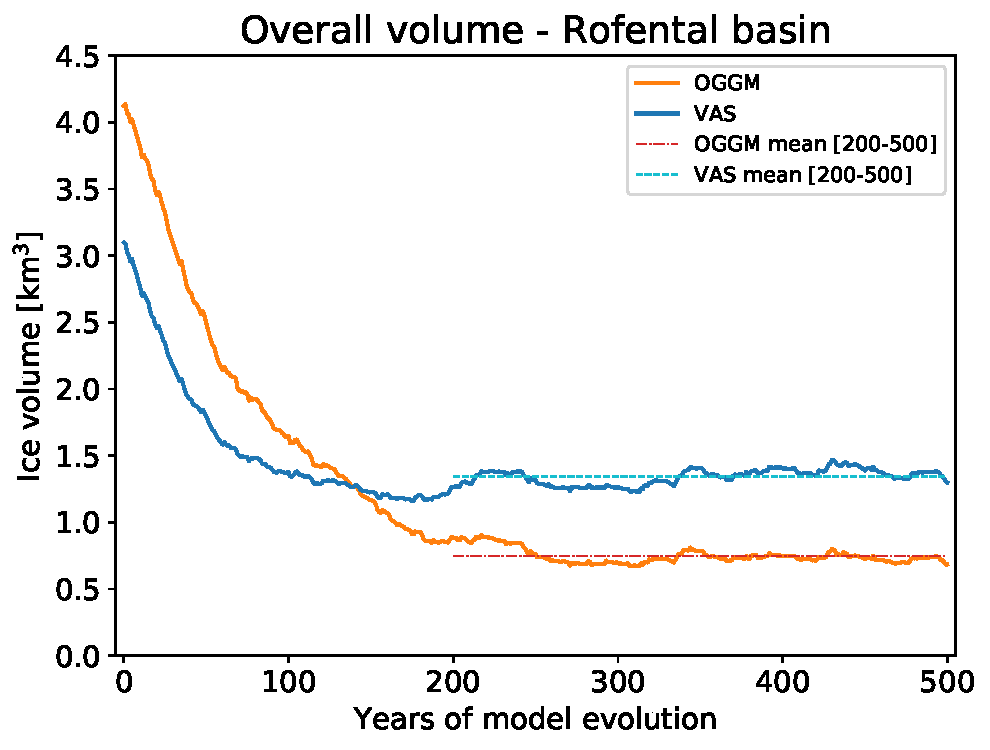
\includegraphics[width=0.75\textwidth]{../plots/rofental.pdf}
         \label{fig:volume_rofental}
      \end{figure}
      The Rofental catchment in the Austrian Alps serves as small scale regional test case. To compare both models I look at the evolution of the basin sum of glacier ice volume over 500 years. Thereby, the mass balance model is driven by randomly drawing climate conditions of single years from the 31-year climate period centered around 1999. This simulates a constant climate similar to the 1884 - 2014 period, using the HistAlp climate data \citep{Auer2007}. Even though the general behavior of both models is comparable, there are still substinatial absolute differences in equilibrium volume. \textbf{And I'm interested in where those differences come from?!}
   \end{boxblock} % End - Rofental commitment run

   %% HEF comparison
   \begin{boxblock}{Comparing the model performances on a single glacier}
      \begin{minipage}[t]{0.45\textwidth}
         \begin{figure}
            \centering
            \includegraphics[width=\textwidth]{../plots/{RGI60-11.00897_area}.pdf}
            \hfill
            \includegraphics[width=\textwidth]{../plots/{RGI60-11.00897_volume}.pdf}
            \label{fig:hef_timeseries}
         \end{figure}
      \end{minipage}
      \hspace{2cm}
      \begin{minipage}[t]{0.45\textwidth}
         \vspace{2cm}
         The Hintereisferner (RGI60-11.00897) example illustrates the different model behaviors for a single glacier. Both models are initialised with the glacier outline of 2003 \citep{RGI}, without any spinup. The models run from 1802 to 2014 using the HistAlp climate data \citep{Auer2007} as input. Hence, the shown glacial evolution is a predominantly \textbf{qualitative result}, not necessarily comparable with the actual evolution of the Hintereisferener.
      \end{minipage}
   \end{boxblock} % END - HEF comparison

   %% Outlook
   \begin{boxblock}{Proof of concept, so what next?!}
      Given that this is just the first implementation step, the (qualitative) results are quite promising. However, some more work is required before deriving any conclusions. This includes the following tasks/questions:
      \begin{itemize}
         \item Glacier length and area as model parameters or actual geometric properties?
         \item Guestimating a start value of the past glacier area for historic runs.
         \item Test the model performance against reference glacier measurements.
         \item Sensibility analysis, given different (non ideal) glacier shapes, slopes, etc.
         \item Regional run for the entire alpine region.
      \end{itemize}
   \end{boxblock} % END - Outlook

   %% References
   \begin{footnotesize}
      \textbf{References:} \\
      \bibliographystyle{ametsoc}
      \bibliography{master}
   \end{footnotesize}
\end{rightcolumn} %% end right column 

\end{columns}
\end{frame}
\end{document}
